% Options for packages loaded elsewhere
\PassOptionsToPackage{unicode}{hyperref}
\PassOptionsToPackage{hyphens}{url}
%
\documentclass[
  ignorenonframetext,
]{beamer}
\usepackage{pgfpages}
\setbeamertemplate{caption}[numbered]
\setbeamertemplate{caption label separator}{: }
\setbeamercolor{caption name}{fg=normal text.fg}
\beamertemplatenavigationsymbolsempty
% Prevent slide breaks in the middle of a paragraph
\widowpenalties 1 10000
\raggedbottom
\setbeamertemplate{part page}{
  \centering
  \begin{beamercolorbox}[sep=16pt,center]{part title}
    \usebeamerfont{part title}\insertpart\par
  \end{beamercolorbox}
}
\setbeamertemplate{section page}{
  \centering
  \begin{beamercolorbox}[sep=12pt,center]{part title}
    \usebeamerfont{section title}\insertsection\par
  \end{beamercolorbox}
}
\setbeamertemplate{subsection page}{
  \centering
  \begin{beamercolorbox}[sep=8pt,center]{part title}
    \usebeamerfont{subsection title}\insertsubsection\par
  \end{beamercolorbox}
}
\AtBeginPart{
  \frame{\partpage}
}
\AtBeginSection{
  \ifbibliography
  \else
    \frame{\sectionpage}
  \fi
}
\AtBeginSubsection{
  \frame{\subsectionpage}
}
\usepackage{lmodern}
\usepackage{amssymb,amsmath}
\usepackage{ifxetex,ifluatex}
\ifnum 0\ifxetex 1\fi\ifluatex 1\fi=0 % if pdftex
  \usepackage[T1]{fontenc}
  \usepackage[utf8]{inputenc}
  \usepackage{textcomp} % provide euro and other symbols
\else % if luatex or xetex
  \usepackage{unicode-math}
  \defaultfontfeatures{Scale=MatchLowercase}
  \defaultfontfeatures[\rmfamily]{Ligatures=TeX,Scale=1}
\fi
% Use upquote if available, for straight quotes in verbatim environments
\IfFileExists{upquote.sty}{\usepackage{upquote}}{}
\IfFileExists{microtype.sty}{% use microtype if available
  \usepackage[]{microtype}
  \UseMicrotypeSet[protrusion]{basicmath} % disable protrusion for tt fonts
}{}
\makeatletter
\@ifundefined{KOMAClassName}{% if non-KOMA class
  \IfFileExists{parskip.sty}{%
    \usepackage{parskip}
  }{% else
    \setlength{\parindent}{0pt}
    \setlength{\parskip}{6pt plus 2pt minus 1pt}}
}{% if KOMA class
  \KOMAoptions{parskip=half}}
\makeatother
\usepackage{xcolor}
\IfFileExists{xurl.sty}{\usepackage{xurl}}{} % add URL line breaks if available
\IfFileExists{bookmark.sty}{\usepackage{bookmark}}{\usepackage{hyperref}}
\hypersetup{
  pdftitle={Module 5: Probabilistic Blocking, Part I},
  pdfauthor={Rebecca C. Steorts},
  hidelinks,
  pdfcreator={LaTeX via pandoc}}
\urlstyle{same} % disable monospaced font for URLs
\newif\ifbibliography
\usepackage{color}
\usepackage{fancyvrb}
\newcommand{\VerbBar}{|}
\newcommand{\VERB}{\Verb[commandchars=\\\{\}]}
\DefineVerbatimEnvironment{Highlighting}{Verbatim}{commandchars=\\\{\}}
% Add ',fontsize=\small' for more characters per line
\usepackage{framed}
\definecolor{shadecolor}{RGB}{248,248,248}
\newenvironment{Shaded}{\begin{snugshade}}{\end{snugshade}}
\newcommand{\AlertTok}[1]{\textcolor[rgb]{0.94,0.16,0.16}{#1}}
\newcommand{\AnnotationTok}[1]{\textcolor[rgb]{0.56,0.35,0.01}{\textbf{\textit{#1}}}}
\newcommand{\AttributeTok}[1]{\textcolor[rgb]{0.77,0.63,0.00}{#1}}
\newcommand{\BaseNTok}[1]{\textcolor[rgb]{0.00,0.00,0.81}{#1}}
\newcommand{\BuiltInTok}[1]{#1}
\newcommand{\CharTok}[1]{\textcolor[rgb]{0.31,0.60,0.02}{#1}}
\newcommand{\CommentTok}[1]{\textcolor[rgb]{0.56,0.35,0.01}{\textit{#1}}}
\newcommand{\CommentVarTok}[1]{\textcolor[rgb]{0.56,0.35,0.01}{\textbf{\textit{#1}}}}
\newcommand{\ConstantTok}[1]{\textcolor[rgb]{0.00,0.00,0.00}{#1}}
\newcommand{\ControlFlowTok}[1]{\textcolor[rgb]{0.13,0.29,0.53}{\textbf{#1}}}
\newcommand{\DataTypeTok}[1]{\textcolor[rgb]{0.13,0.29,0.53}{#1}}
\newcommand{\DecValTok}[1]{\textcolor[rgb]{0.00,0.00,0.81}{#1}}
\newcommand{\DocumentationTok}[1]{\textcolor[rgb]{0.56,0.35,0.01}{\textbf{\textit{#1}}}}
\newcommand{\ErrorTok}[1]{\textcolor[rgb]{0.64,0.00,0.00}{\textbf{#1}}}
\newcommand{\ExtensionTok}[1]{#1}
\newcommand{\FloatTok}[1]{\textcolor[rgb]{0.00,0.00,0.81}{#1}}
\newcommand{\FunctionTok}[1]{\textcolor[rgb]{0.00,0.00,0.00}{#1}}
\newcommand{\ImportTok}[1]{#1}
\newcommand{\InformationTok}[1]{\textcolor[rgb]{0.56,0.35,0.01}{\textbf{\textit{#1}}}}
\newcommand{\KeywordTok}[1]{\textcolor[rgb]{0.13,0.29,0.53}{\textbf{#1}}}
\newcommand{\NormalTok}[1]{#1}
\newcommand{\OperatorTok}[1]{\textcolor[rgb]{0.81,0.36,0.00}{\textbf{#1}}}
\newcommand{\OtherTok}[1]{\textcolor[rgb]{0.56,0.35,0.01}{#1}}
\newcommand{\PreprocessorTok}[1]{\textcolor[rgb]{0.56,0.35,0.01}{\textit{#1}}}
\newcommand{\RegionMarkerTok}[1]{#1}
\newcommand{\SpecialCharTok}[1]{\textcolor[rgb]{0.00,0.00,0.00}{#1}}
\newcommand{\SpecialStringTok}[1]{\textcolor[rgb]{0.31,0.60,0.02}{#1}}
\newcommand{\StringTok}[1]{\textcolor[rgb]{0.31,0.60,0.02}{#1}}
\newcommand{\VariableTok}[1]{\textcolor[rgb]{0.00,0.00,0.00}{#1}}
\newcommand{\VerbatimStringTok}[1]{\textcolor[rgb]{0.31,0.60,0.02}{#1}}
\newcommand{\WarningTok}[1]{\textcolor[rgb]{0.56,0.35,0.01}{\textbf{\textit{#1}}}}
\usepackage{longtable,booktabs}
\usepackage{caption}
% Make caption package work with longtable
\makeatletter
\def\fnum@table{\tablename~\thetable}
\makeatother
\usepackage{graphicx,grffile}
\makeatletter
\def\maxwidth{\ifdim\Gin@nat@width>\linewidth\linewidth\else\Gin@nat@width\fi}
\def\maxheight{\ifdim\Gin@nat@height>\textheight\textheight\else\Gin@nat@height\fi}
\makeatother
% Scale images if necessary, so that they will not overflow the page
% margins by default, and it is still possible to overwrite the defaults
% using explicit options in \includegraphics[width, height, ...]{}
\setkeys{Gin}{width=\maxwidth,height=\maxheight,keepaspectratio}
% Set default figure placement to htbp
\makeatletter
\def\fps@figure{htbp}
\makeatother
\setlength{\emergencystretch}{3em} % prevent overfull lines
\providecommand{\tightlist}{%
  \setlength{\itemsep}{0pt}\setlength{\parskip}{0pt}}
\setcounter{secnumdepth}{-\maxdimen} % remove section numbering
% Custom definitions
% To use this customization file, insert the line "\input{custom}" in the header of the tex file.

% Formatting




% Packages

\setbeamertemplate{navigation symbols}{}
\setbeamertemplate{footline}[page number]

 \usepackage{amssymb,latexsym}
\usepackage{amssymb,amsfonts,amsmath,latexsym,amsthm, bm}
%\usepackage[usenames,dvipsnames]{color}
%\usepackage[]{graphicx}
%\usepackage[space]{grffile}
\usepackage{mathrsfs}   % fancy math font
% \usepackage[font=small,skip=0pt]{caption}
%\usepackage[skip=0pt]{caption}
%\usepackage{subcaption}
%\usepackage{verbatim}
%\usepackage{url}
%\usepackage{bm}
\usepackage{dsfont}
\usepackage{multirow}
%\usepackage{extarrows}
%\usepackage{multirow}
%% \usepackage{wrapfig}
%% \usepackage{epstopdf}
%\usepackage{rotating}
%\usepackage{tikz}
%\usetikzlibrary{fit}					% fitting shapes to coordinates
%\usetikzlibrary{backgrounds}	% drawing the background after the foreground


% \usepackage[dvipdfm,colorlinks,citecolor=blue,linkcolor=blue,urlcolor=blue]{hyperref}
%\usepackage[colorlinks,citecolor=blue,linkcolor=blue,urlcolor=blue]{hyperref}
%%\usepackage{hyperref}
%\usepackage[authoryear,round]{natbib}


%  Theorems, etc.

%\theoremstyle{plain}
%\newtheorem{theorem}{Theorem}[section]
%\newtheorem{corollary}[theorem]{Corollary}
%\newtheorem{lemma}[theorem]{Lemma}
%\newtheorem{proposition}[theorem]{Proposition}
%\newtheorem{condition}[theorem]{Condition}
% \newtheorem{conditions}[theorem]{Conditions}

%\theoremstyle{definition}
%\newtheorem{definition}[theorem]{Definition}
%% \newtheorem*{unnumbered-definition}{Definition}
%\newtheorem{example}[theorem]{Example}
%\theoremstyle{remark}
%\newtheorem*{remark}{Remark}
%\numberwithin{equation}{section}




% Document-specific shortcuts
\newcommand{\btheta}{{\bm\theta}}
\newcommand{\bbtheta}{{\pmb{\bm\theta}}}

\newcommand{\commentary}[1]{\ifx\showcommentary\undefined\else \emph{#1}\fi}

\newcommand{\term}[1]{\textit{\textbf{#1}}}

% Math shortcuts

% Probability distributions
\DeclareMathOperator*{\Exp}{Exp}
\DeclareMathOperator*{\TExp}{TExp}
\DeclareMathOperator*{\Bernoulli}{Bernoulli}
\DeclareMathOperator*{\Beta}{Beta}
\DeclareMathOperator*{\Ga}{Gamma}
\DeclareMathOperator*{\TGamma}{TGamma}
\DeclareMathOperator*{\Poisson}{Poisson}
\DeclareMathOperator*{\Binomial}{Binomial}
\DeclareMathOperator*{\NormalGamma}{NormalGamma}
\DeclareMathOperator*{\InvGamma}{InvGamma}
\DeclareMathOperator*{\Cauchy}{Cauchy}
\DeclareMathOperator*{\Uniform}{Uniform}
\DeclareMathOperator*{\Gumbel}{Gumbel}
\DeclareMathOperator*{\Pareto}{Pareto}
\DeclareMathOperator*{\Mono}{Mono}
\DeclareMathOperator*{\Geometric}{Geometric}
\DeclareMathOperator*{\Wishart}{Wishart}

% Math operators
\DeclareMathOperator*{\argmin}{arg\,min}
\DeclareMathOperator*{\argmax}{arg\,max}
\DeclareMathOperator*{\Cov}{Cov}
\DeclareMathOperator*{\diag}{diag}
\DeclareMathOperator*{\median}{median}
\DeclareMathOperator*{\Vol}{Vol}

% Math characters
\newcommand{\R}{\mathbb{R}}
\newcommand{\Z}{\mathbb{Z}}
\newcommand{\E}{\mathbb{E}}
\renewcommand{\Pr}{\mathbb{P}}
\newcommand{\I}{\mathds{1}}
\newcommand{\V}{\mathbb{V}}

\newcommand{\A}{\mathcal{A}}
%\newcommand{\C}{\mathcal{C}}
\newcommand{\D}{\mathcal{D}}
\newcommand{\Hcal}{\mathcal{H}}
\newcommand{\M}{\mathcal{M}}
\newcommand{\N}{\mathcal{N}}
\newcommand{\X}{\mathcal{X}}
\newcommand{\Zcal}{\mathcal{Z}}
\renewcommand{\P}{\mathcal{P}}

\newcommand{\T}{\mathtt{T}}
\renewcommand{\emptyset}{\varnothing}


% Miscellaneous commands
\newcommand{\iid}{\stackrel{\mathrm{iid}}{\sim}}
\newcommand{\matrixsmall}[1]{\bigl(\begin{smallmatrix}#1\end{smallmatrix} \bigr)}

\newcommand{\items}[1]{\begin{itemize} #1 \end{itemize}}

\newcommand{\todo}[1]{\emph{\textcolor{red}{(#1)}}}

\newcommand{\branch}[4]{
\left\{
	\begin{array}{ll}
		#1  & \mbox{if } #2 \\
		#3 & \mbox{if } #4
	\end{array}
\right.
}

% approximately proportional to
\def\app#1#2{%
  \mathrel{%
    \setbox0=\hbox{$#1\sim$}%
    \setbox2=\hbox{%
      \rlap{\hbox{$#1\propto$}}%
      \lower1.3\ht0\box0%
    }%
    \raise0.25\ht2\box2%
  }%
}
\def\approxprop{\mathpalette\app\relax}

% \newcommand{\approptoinn}[2]{\mathrel{\vcenter{
  % \offinterlineskip\halign{\hfil$##$\cr
    % #1\propto\cr\noalign{\kern2pt}#1\sim\cr\noalign{\kern-2pt}}}}}

% \newcommand{\approxpropto}{\mathpalette\approptoinn\relax}

\title{Module 5: Probabilistic Blocking, Part I}
\author{Rebecca C. Steorts}
\date{}

\begin{document}
\frame{\titlepage}

\begin{frame}{Agenda}
\protect\hypertarget{agenda}{}

\begin{itemize}
\tightlist
\item
  Data Cleaning Pipeline
\item
  Blocking
\item
  Probabilistic Blocking
\item
  Locality Sensitive Hashing (LSH)
\item
  Jaccard Similarity
\item
  Shingling
\item
  Putting it together
\item
  Limitations
\end{itemize}

\end{frame}

\begin{frame}[fragile]{Load R packages}
\protect\hypertarget{load-r-packages}{}

\begin{Shaded}
\begin{Highlighting}[]
\KeywordTok{library}\NormalTok{(RecordLinkage)}
\KeywordTok{library}\NormalTok{(blink)}
\KeywordTok{library}\NormalTok{(knitr)}
\KeywordTok{library}\NormalTok{(cora)}
\KeywordTok{library}\NormalTok{(ggplot2)}
\end{Highlighting}
\end{Shaded}

\end{frame}

\begin{frame}{Data Cleaning Pipeline}
\protect\hypertarget{data-cleaning-pipeline}{}

\begin{figure}
  \begin{center}
    \includegraphics[width=\textwidth]{finalFigures/pipeline}
    \caption{Data cleaning pipeline.}
    \end{center}
\end{figure}

\end{frame}

\begin{frame}{Blocking}
\protect\hypertarget{blocking}{}

\begin{figure}
  \begin{center}
    \includegraphics[width=\textwidth]{finalFigures/block.png}
    \caption{Left: All to all record comparison. Right: Example of resulting blocking partitions. }
    \end{center}
\end{figure}

\end{frame}

\begin{frame}{LSH}
\protect\hypertarget{lsh}{}

Locality sensitive hashing (LSH) is a fast method of blocking for record
linkage that orginates from the computer science literature.

\end{frame}

\begin{frame}{Finding similar records}
\protect\hypertarget{finding-similar-records}{}

Our goal is to find \emph{similar} records, where the records are
assumed to be strings \vfill

How do we define \emph{similar}? \vfill

\end{frame}

\begin{frame}{Jaccard similarity}
\protect\hypertarget{jaccard-similarity}{}

We will work with the \emph{Jaccard similarity}: \[
Jac(S, T) = \frac{\mid S \cap T\mid}{\mid S \cup T \mid}.
\]

\begin{figure}[h]
\centering
\includegraphics[width=.5\textwidth]{finalFigures/jaccard}
\caption{Two sets S and T with Jaccard similarity 3/7. The two sets share 3 elements in common, and there are 7 elements in total.}
\label{fig:jaccard}
\end{figure}

\end{frame}

\begin{frame}{How to represent data as sets?}
\protect\hypertarget{how-to-represent-data-as-sets}{}

We want to talk about the similarity of our data
(records)\(\Rightarrow\) we need to compare sets of records!

\begin{itemize}
\tightlist
\item
  We can construct a set of \textbf{short strings} from the data \vfill
\item
  This is useful because similar datasets will have many common elements
  (common short strings) \vfill
\item
  We can do construct these short strings using \emph{shingling} \vfill
\end{itemize}

\end{frame}

\begin{frame}{\(k\)-shingling (how-to)}
\protect\hypertarget{k-shingling-how-to}{}

\begin{enumerate}
\tightlist
\item
  Think of the data set as a string of characters \vfill
\item
  A \(k\)-shingle (k-gram) is any sub-string (word) of length \(k\)
  found within the a record of the data set \vfill
\item
  Associate with each data set the set of \(k\)-shingles that appear one
  or more times \vfill
\end{enumerate}

\end{frame}

\begin{frame}{Let's try}
\protect\hypertarget{lets-try}{}

Suppose our data set is the string ``Hello world'', then

\begin{itemize}
\tightlist
\item
  the set of \(2\)-shingles is
  \(\{\text{he, el, ll, lo, ow, wo, or, rl, ld}\}\) \vfill
\item
  the set of \(3\)-shingles is
  \(\{\text{hel, ell, llo, low, owo, wor, orl, rld}\}\) \vfill
\end{itemize}

\end{frame}

\begin{frame}[fragile]{Your turn}
\protect\hypertarget{your-turn}{}

We have the following two records:

\begin{Shaded}
\begin{Highlighting}[]
\CommentTok{# load RL data}
\KeywordTok{data}\NormalTok{(}\StringTok{"RLdata500"}\NormalTok{)}

\CommentTok{# select only 2 records}
\NormalTok{records <-}\StringTok{ }\NormalTok{RLdata500[}\DecValTok{129}\OperatorTok{:}\DecValTok{130}\NormalTok{, }\KeywordTok{c}\NormalTok{(}\DecValTok{1}\NormalTok{,}\DecValTok{3}\NormalTok{)]}
\KeywordTok{names}\NormalTok{(records) <-}\StringTok{ }\KeywordTok{c}\NormalTok{(}\StringTok{"First name"}\NormalTok{, }\StringTok{"Last name"}\NormalTok{)}

\CommentTok{# inspect records}
\KeywordTok{kable}\NormalTok{(records)}
\end{Highlighting}
\end{Shaded}

\begin{longtable}[]{@{}lll@{}}
\toprule
& First name & Last name\tabularnewline
\midrule
\endhead
129 & MICHAEL & VOGEL\tabularnewline
130 & MICHAEL & MEYER\tabularnewline
\bottomrule
\end{longtable}

\end{frame}

\begin{frame}{Your turn (continued)}
\protect\hypertarget{your-turn-continued}{}

\begin{enumerate}
\tightlist
\item
  Compute the \(2\)-shingles for each record \vfill
\item
  Using Jaccard similarity, how similar are they? \vfill
\item
  What do you learn from this exercise?
\end{enumerate}

\end{frame}

\begin{frame}{Your turn solution}
\protect\hypertarget{your-turn-solution}{}

\textbf{Do this on your own and compare with a partner.}

\end{frame}

\begin{frame}[fragile]{Useful packages/functions in \texttt{R}}
\protect\hypertarget{useful-packagesfunctions-in-r}{}

From the exercise, you should have learned that we don't want to do this
by hand!

Here are some useful packages in \texttt{R} that can help us!

\vline

\begin{Shaded}
\begin{Highlighting}[]
\KeywordTok{library}\NormalTok{(textreuse) }\CommentTok{# text reuse/document similarity}
\KeywordTok{library}\NormalTok{(tokenizers) }\CommentTok{# shingles}
\end{Highlighting}
\end{Shaded}

\end{frame}

\begin{frame}[fragile]{Shingling}
\protect\hypertarget{shingling}{}

We can use the following functions to create \(k\)-shingles and
calculate Jaccard similarity for our data

\vline

\begin{Shaded}
\begin{Highlighting}[]
\CommentTok{# get k-shingles}
\KeywordTok{tokenize_character_shingles}\NormalTok{(x, n)}

\CommentTok{# calculate jaccard similarity for two sets}
\KeywordTok{jaccard_similarity}\NormalTok{(a, b) }
\end{Highlighting}
\end{Shaded}

\end{frame}

\begin{frame}{Citation Data Set}
\protect\hypertarget{citation-data-set}{}

Research paper headers and citations, with information on authors,
title, institutions, venue, date, page numbers and several other fields.

\end{frame}

\begin{frame}[fragile]{Citation Data Set}
\protect\hypertarget{citation-data-set-1}{}

\begin{Shaded}
\begin{Highlighting}[]
\KeywordTok{data}\NormalTok{(cora) }\CommentTok{# load the cora data set}
\KeywordTok{str}\NormalTok{(cora) }\CommentTok{# structure of cora}
\end{Highlighting}
\end{Shaded}

\begin{verbatim}
## 'data.frame':    1879 obs. of  16 variables:
##  $ id         : int  1 2 3 4 5 6 7 8 9 10 ...
##  $ title      : 'noquote' chr  "Inganas and M.R" NA NA NA ...
##  $ book_title : 'noquote' chr  NA NA NA NA ...
##  $ authors    : 'noquote' chr  "M. Ahlskog, J. Paloheimo, H. Stubb, P. Dyreklev, M. Fahlman, O" "M. Ahlskog, J. Paloheimo, H. Stubb, P. Dyreklev, M. Fahlman, O. Inganas and M.R.   Andersson" "M. Ahlskog, J. Paloheimo, H. Stubb, P. Dyreklev, M. Fahlman, O.  Inganas and M.R.  Andersson" "M. Ahlskog, J. Paloheimo, H. Stubb, P. Dyreklev, M. Fahlman, O. Inganas and M.R. Andersson" ...
##  $ address    : 'noquote' chr  NA NA NA NA ...
##  $ date       : 'noquote' chr  "1994" "1994" "1994" "1994" ...
##  $ year       : 'noquote' chr  NA NA NA NA ...
##  $ editor     : 'noquote' chr  NA NA NA NA ...
##  $ journal    : 'noquote' chr  "Andersson, J Appl. Phys." "JAppl. Phys." "J Appl. Phys." "J Appl.Phys." ...
##  $ volume     : 'noquote' chr  "76" "76" "76" "76" ...
##  $ pages      : 'noquote' chr  "893" "893" "893" "893" ...
##  $ publisher  : 'noquote' chr  NA NA NA NA ...
##  $ institution: 'noquote' chr  NA NA NA NA ...
##  $ type       : 'noquote' chr  NA NA NA NA ...
##  $ tech       : 'noquote' chr  NA NA NA NA ...
##  $ note       : 'noquote' chr  NA NA NA NA ...
\end{verbatim}

\end{frame}

\begin{frame}[fragile]{Your turn}
\protect\hypertarget{your-turn-1}{}

Using the \texttt{title}, \texttt{authors}, and \texttt{journal} fields
in the \texttt{cora} dataset,

\vfill

\begin{enumerate}
\tightlist
\item
  Get the \(3\)-shingles for each record (\textbf{hint:} use
  \texttt{tokenize\_character\_shingles}) \vfill
\item
  Obtain the Jaccard similarity between each pair of records
  (\textbf{hint:} use \texttt{jaccard\_similarity}) \vfill
\end{enumerate}

\end{frame}

\begin{frame}[fragile]{Your turn (solution)}
\protect\hypertarget{your-turn-solution-1}{}

\small

\begin{Shaded}
\begin{Highlighting}[]
\CommentTok{# get only the columns we want}
\CommentTok{# number of records}
\NormalTok{n <-}\StringTok{ }\KeywordTok{nrow}\NormalTok{(cora) }
\CommentTok{# create id column}
\NormalTok{dat <-}\StringTok{ }\KeywordTok{data.frame}\NormalTok{(}\DataTypeTok{id =} \KeywordTok{seq_len}\NormalTok{(n)) }
\CommentTok{# get columns we want}
\NormalTok{dat <-}\StringTok{ }\KeywordTok{cbind}\NormalTok{(dat, cora[, }\KeywordTok{c}\NormalTok{(}\StringTok{"title"}\NormalTok{, }\StringTok{"authors"}\NormalTok{, }\StringTok{"journal"}\NormalTok{)])}

\CommentTok{# 1. paste the columns together and tokenize for each record}
\NormalTok{shingles <-}\StringTok{ }\KeywordTok{apply}\NormalTok{(dat, }\DecValTok{1}\NormalTok{, }\ControlFlowTok{function}\NormalTok{(x) \{}
  \CommentTok{# tokenize strings}
  \KeywordTok{tokenize_character_shingles}\NormalTok{(}\KeywordTok{paste}\NormalTok{(x[}\OperatorTok{-}\DecValTok{1}\NormalTok{], }\DataTypeTok{collapse=}\StringTok{" "}\NormalTok{), }\DataTypeTok{n =} \DecValTok{3}\NormalTok{)[[}\DecValTok{1}\NormalTok{]]}
\NormalTok{\})}
\end{Highlighting}
\end{Shaded}

\end{frame}

\begin{frame}[fragile]{Your turn (solution)}
\protect\hypertarget{your-turn-solution-2}{}

\small

\begin{Shaded}
\begin{Highlighting}[]
\CommentTok{# 2. Jaccard similarity between pairs}
\CommentTok{# empty holder for similarities}
\NormalTok{jaccard <-}\StringTok{ }\KeywordTok{expand.grid}\NormalTok{(}\DataTypeTok{record1 =} \KeywordTok{seq_len}\NormalTok{(n), }
                       \DataTypeTok{record2 =} \KeywordTok{seq_len}\NormalTok{(n))}

\CommentTok{# don't need to compare the same things twice}
\NormalTok{jaccard <-}\StringTok{ }\NormalTok{jaccard[jaccard}\OperatorTok{$}\NormalTok{record1 }\OperatorTok{<}\StringTok{ }\NormalTok{jaccard}\OperatorTok{$}\NormalTok{record2,]}

\NormalTok{time <-}\StringTok{ }\KeywordTok{Sys.time}\NormalTok{() }\CommentTok{# for timing comparison}
\NormalTok{jaccard}\OperatorTok{$}\NormalTok{similarity <-}\StringTok{ }\KeywordTok{apply}\NormalTok{(jaccard, }\DecValTok{1}\NormalTok{, }\ControlFlowTok{function}\NormalTok{(pair) \{}
  \CommentTok{# get jaccard for each pair}
  \KeywordTok{jaccard_similarity}\NormalTok{(shingles[[pair[}\DecValTok{1}\NormalTok{]]], shingles[[pair[}\DecValTok{2}\NormalTok{]]]) }
\NormalTok{\})}
\CommentTok{# timing}
\NormalTok{time <-}\StringTok{ }\KeywordTok{difftime}\NormalTok{(}\KeywordTok{Sys.time}\NormalTok{(), time, }\DataTypeTok{units =} \StringTok{"secs"}\NormalTok{) }
\end{Highlighting}
\end{Shaded}

\normalsize

This took took \(108.7\) seconds \(\approx 1.81\) minutes

\end{frame}

\begin{frame}[fragile]{Your turn (solution, cont'd)}
\protect\hypertarget{your-turn-solution-contd}{}

\begin{Shaded}
\begin{Highlighting}[]
\CommentTok{# plot the jaccard similarities for each pair of records}
\KeywordTok{ggplot}\NormalTok{(jaccard) }\OperatorTok{+}
\StringTok{  }\KeywordTok{geom_raster}\NormalTok{(}\KeywordTok{aes}\NormalTok{(}\DataTypeTok{x =}\NormalTok{ record1, }\DataTypeTok{y =}\NormalTok{ record2, }
                  \DataTypeTok{fill=}\NormalTok{similarity)) }\OperatorTok{+}
\StringTok{  }\KeywordTok{theme}\NormalTok{(}\DataTypeTok{aspect.ratio =} \DecValTok{1}\NormalTok{) }\OperatorTok{+}
\StringTok{  }\KeywordTok{scale_fill_gradient}\NormalTok{(}\StringTok{"Jaccard similarity"}\NormalTok{) }\OperatorTok{+}
\StringTok{  }\KeywordTok{xlab}\NormalTok{(}\StringTok{"Record id"}\NormalTok{) }\OperatorTok{+}\StringTok{ }\KeywordTok{ylab}\NormalTok{(}\StringTok{"Record id"}\NormalTok{)}
\end{Highlighting}
\end{Shaded}

\begin{figure}
\centering
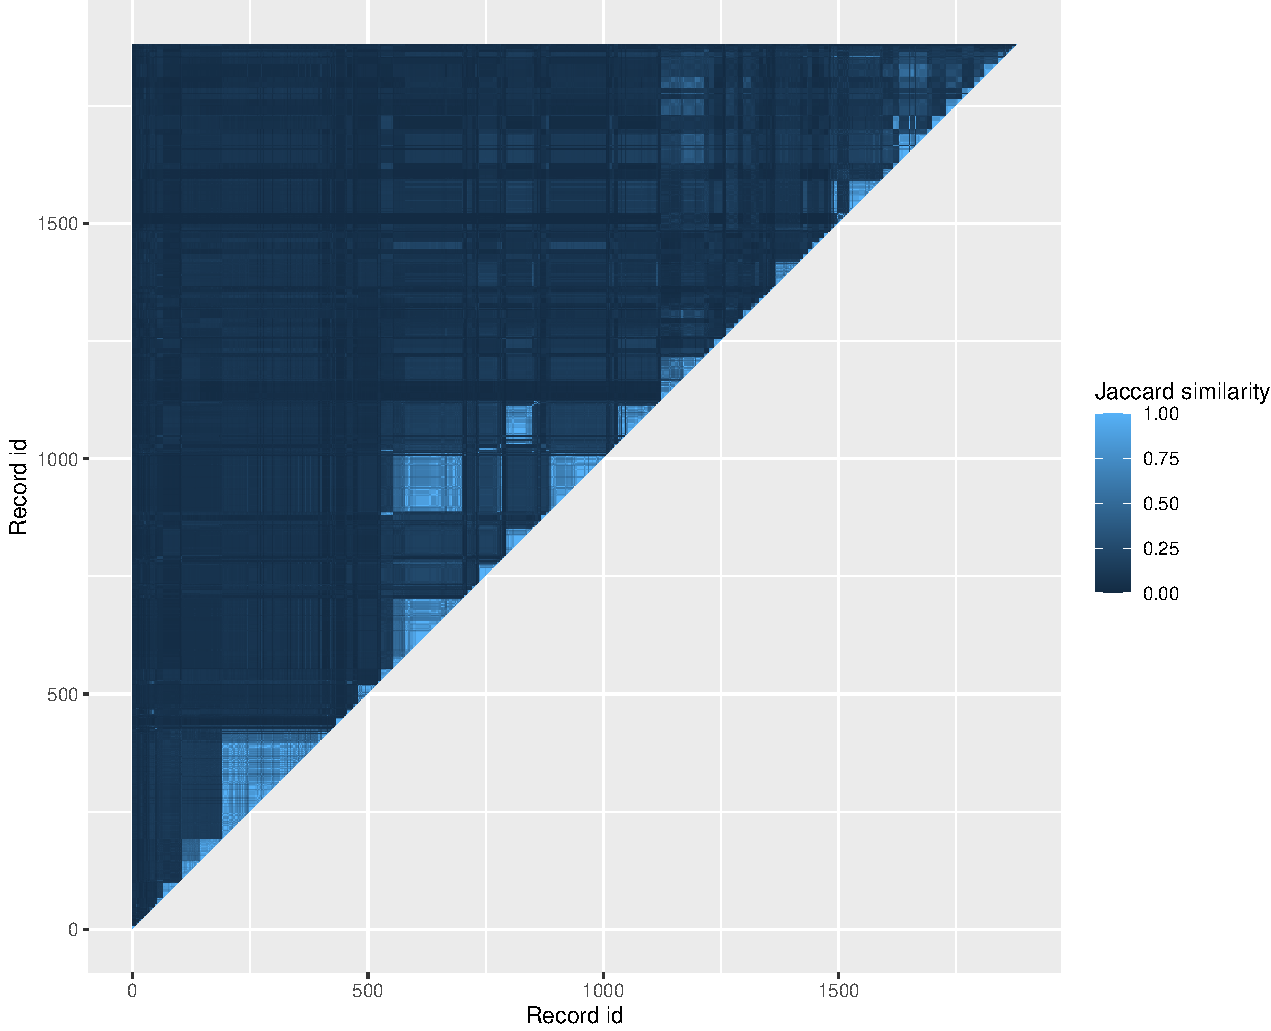
\includegraphics{probabilistic-blocking-partI_files/figure-beamer/your-turn2-plot-1.pdf}
\caption{Jaccard similarity for each pair of records. Light blue
indicates the two records are more similar and dark blue indicates less
similar.}
\end{figure}

\end{frame}

\begin{frame}{Your turn (solution, cont'd)}
\protect\hypertarget{your-turn-solution-contd-1}{}

\begin{figure}
\centering
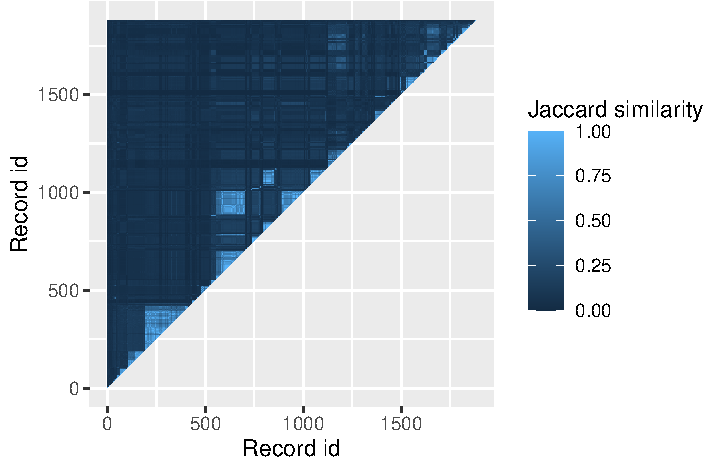
\includegraphics{probabilistic-blocking-partI_files/figure-beamer/your-turn2-plot-again-1.pdf}
\caption{Jaccard similarity for each pair of records. Light blue
indicates the two records are more similar and dark blue indicates less
similar.}
\end{figure}

\end{frame}

\begin{frame}{Summary}
\protect\hypertarget{summary}{}

For a data set of size \(n\), the number of comparisons we must compute
is \[\frac{n(n-1)}{2}.\]

\vfill

For our set of records, we needed to compute \(1,764,381\) comparisons
\vfill For very large data sets, we need something faster (where we
filter out records that are not similar). \vfill A better approach for
data sets of any realistic size is to use \emph{hashing}, which we will
look at next time. \vfill

\end{frame}

\end{document}
